\section{Introduction}
\label{sec:intro}

Deployed runtimes for computer-use agents increasingly integrate visual desktop control (GUI), command-line and code execution (CLI/code), browsers, and external tools within a single agent loop~\citep{openai2025chatgptagent,anthropic2025claudecode,openai2026codexagent,anthropic2026cowork,peekaboo2026}. This integration reflects the demands of production workflows, where agents must coordinate multiple interfaces. Figure~\ref{fig:paradigm} illustrates three examples to show this requirement: solving such workflows requires agents to interleave GUI-side observations with CLI/code-side inspection, modification, and verification. These channels are complementary rather than interchangeable: GUIs expose rendered and transient interactive state, such as canvases, spatial layout, dialogs, and visual feedback, whereas CLI/code interfaces expose structured, scriptable, and persistent state, such as source files, configurations, logs, artifacts, and service status. Evaluation should therefore shift to cross-interface orchestration: whether an agent can coordinate GUI, CLI/code, browsers, and external tools within one workflow.

\begin{figure*}[t]
\centering
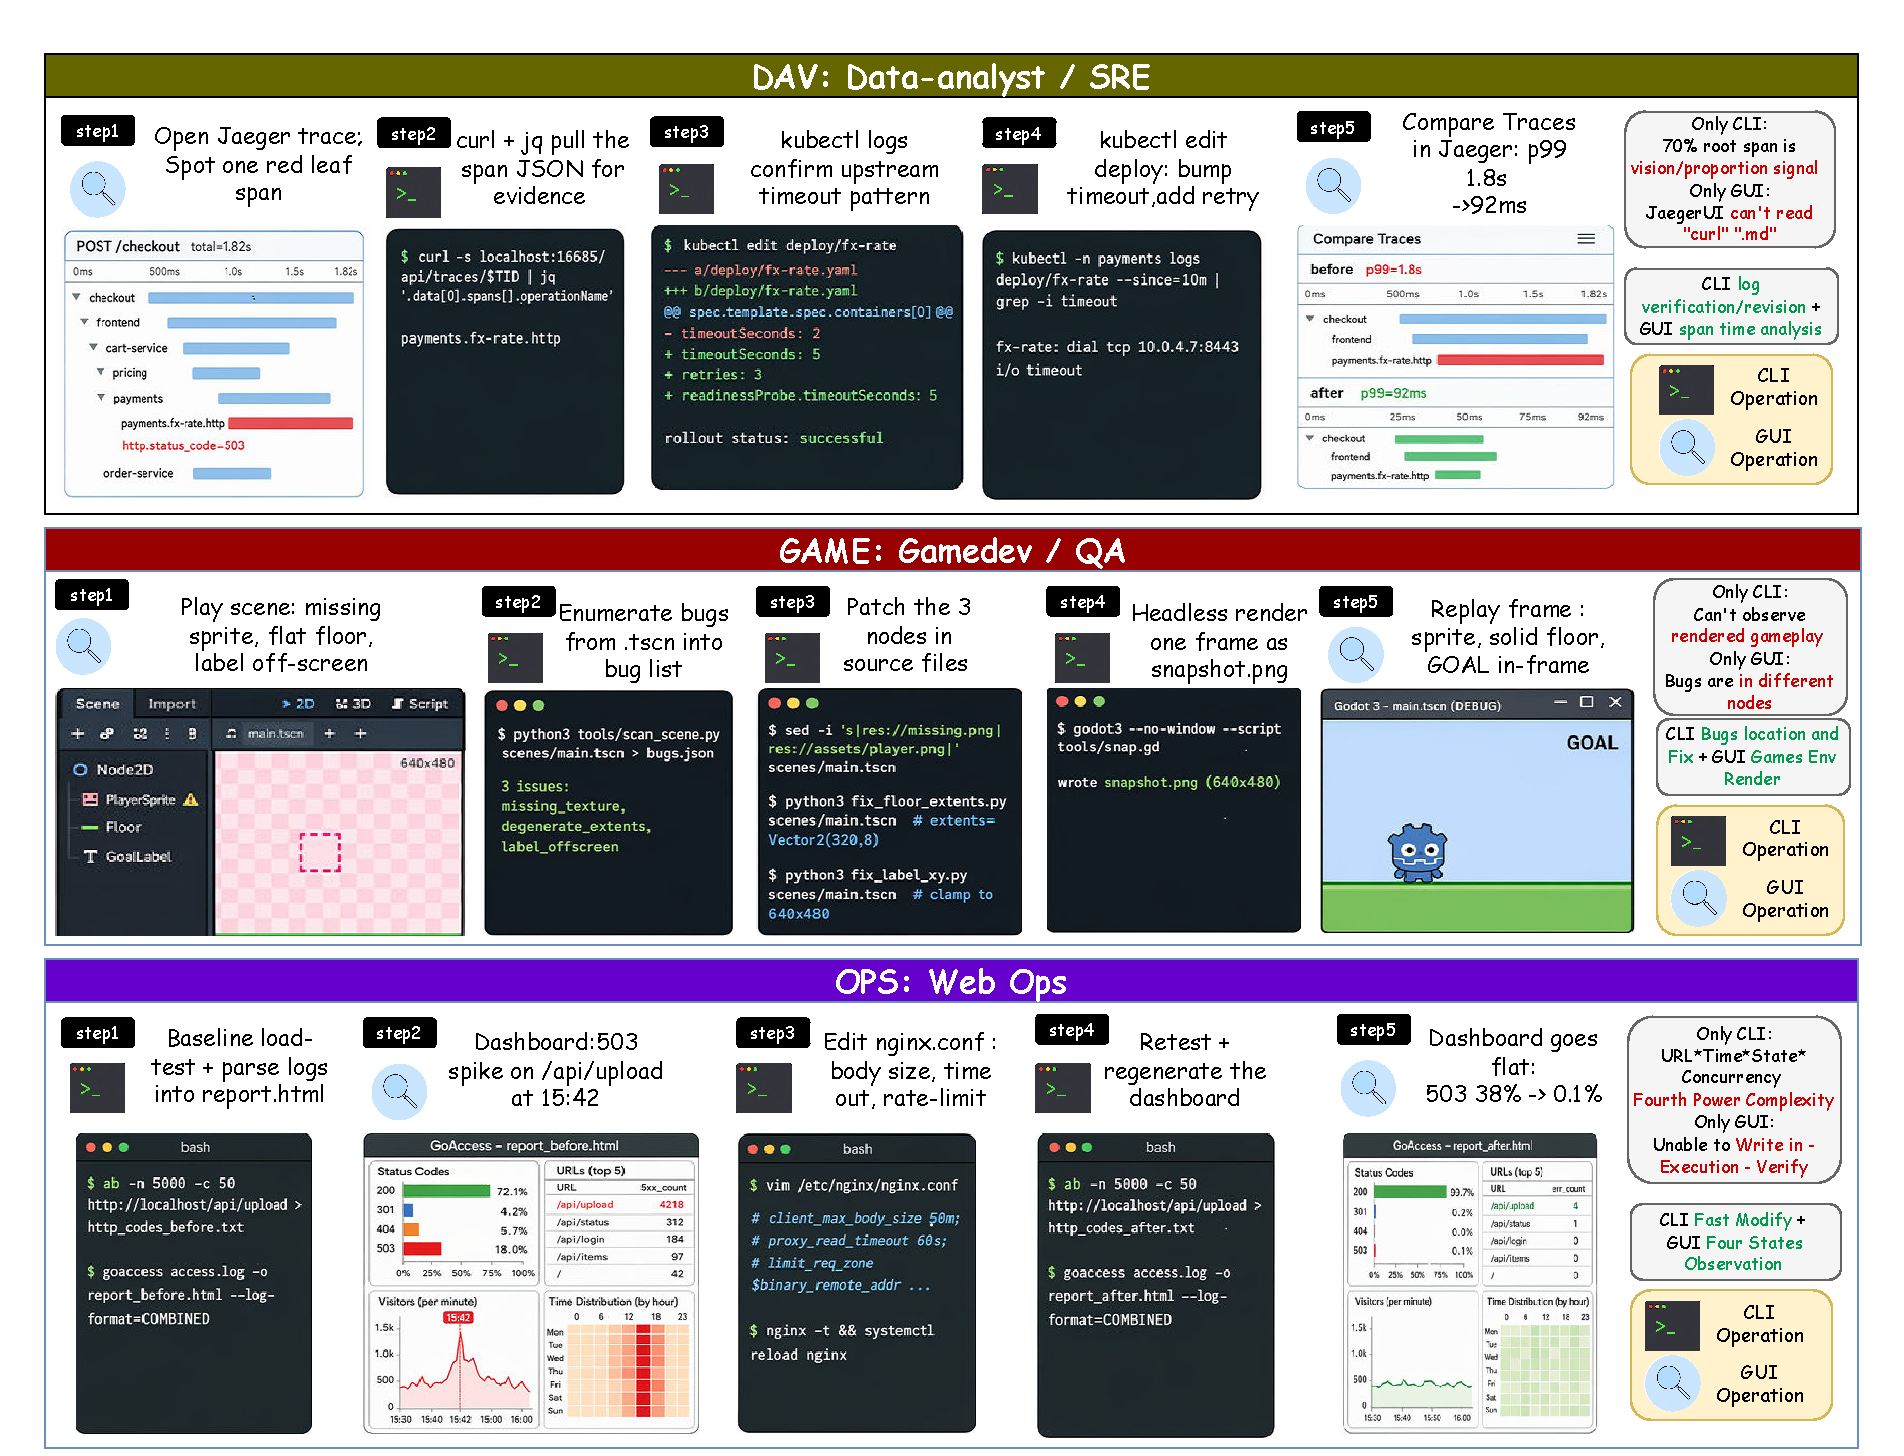
\includegraphics[width=\textwidth]{figures/fig_casestudy_3panel.pdf}
\caption{\textbf{Three real-world workflows requiring interleaved hybrid interfaces.} (DAV) Diagnosing a Jaeger trace span by inspecting its shape, then patching the upstream timeout via \texttt{kubectl}; (GAME) playing a desktop game to localize a sprite/physics bug, then patching the scene-graph source; (OPS) catching a 503 spike on a Web Ops dashboard, editing \texttt{nginx.conf}, and re-checking the dashboard. Each step alternates between a GUI signal that no API exposes and a CLI/code change that no screenshot can produce.}
\label{fig:paradigm}
\end{figure*}

However, as shown in Table~\ref{tab:positioning}, existing CUA benchmarks have not directly evaluated this coordination. GUI/OS benchmarks~\citep{xie2024osworld,bonatti2024waa,rawles2025androidworld,koh2024visualwebarena,zhou2024webarena} and CLI/coding benchmarks~\citep{terminalbench2025,chu2026terminalworld,cheng2026terminalworldsynth} each expose only a single channel, so the hybrid workflows remain unreachable; worse, on such GUI benchmarks the CLI channel can reach the same target states just as effectively (e.g.\ on \osworld{} a pixel-blind CLI agent matches a vision agent's accuracy at half the steps, Appendix~\ref{app:cli-osworld}); multi-interface benchmarks~\citep{yan2025mcpworld,jia2025osworldmcp,aggarwal2025pwp,sun2026scienceboard,hao2026cocoabench,shi2026saasbench} jointly expose GUI and CLI/MCP, but most tasks remain solvable through a single channel, making the extra channel a convenience rather than a requirement; and Claw-class benchmarks~\citep{ding2026wildclawbench,zhang2026clawbench,chu2026terminalworld,ye2026clawEval,li2026clawenvkit,meng2026clawmark,kilocode2026pinchbench} evaluate real-world, long-horizon user tasks inside deployed agent runtimes, but inherit a CLI-only scope with no GUI interface.

To address this gap, we propose \Eyeson{}, a benchmark for long-horizon hybrid-interface computer use. It contains 114 tasks across 8 real-world work domains, sourced from real user requests submitted to deployed open-source agent runtimes, with traceable provenance. Each task requires agents to combine GUI observations/actions with CLI/code-side operations within one trajectory.

We evaluate these tasks in deployed agent runtimes rather than a custom simulator. Starting from \textsc{OpenClaw}~\citep{openclaw2025}, we add a minimal GUI plugin: one perception tool (\texttt{screenshot}) and nine atomic actuation primitives (\texttt{click}, \texttt{drag}, \texttt{scroll}, \texttt{type}, \texttt{keypress}, etc.). These tools are exposed alongside existing terminal, file, code, and browser tools. The same plugin is ported to \textsc{Codex CLI}~\citep{openai2026codexagent}, \textsc{Claude Code}~\citep{anthropic2025claudecode}, and \textsc{Hermes}~\citep{hermes2025}, enabling cross-harness evaluation.

To make the evaluation reliable, we further propose a trajectory-aware agentic judge: an isolated subprocess that re-fetches evidence over multiple turns using file, image, and shell tools, because final deliverables can be synthesized, hard-coded, or protocol-violating. The judge decomposes each deliverable into verifiable clauses, scores eight process and outcome dimensions, and zeroes rollouts when high-confidence shortcut evidence is found. This evaluation protocol is designed to measure successful cross-interface execution, not merely plausible final artifacts.

Experiments show that \Eyeson{} remains far from saturated. On the fixed \textsc{OpenClaw} harness, Claude Opus 4.7 reaches 35.1\% PassRate, with GPT-5.5 at 33.3\%; across deployed harnesses, the best model--runtime pairing (Claude Opus 4.7 + \textsc{Claude Code}) reaches 41.2\%. These scores are substantially lower than the $>$78\% reported for frontier backbones on \osworld{}-Verified. The interface ablation shows that GUI-only and CLI-only settings stay at or below 3.5\%. Trajectory-aware judging corrects PassRate, reducing GPT-5.5 from 53.5\% to an audited 33.3\%. Together, these results show that current models and runtimes still struggle with long-horizon orchestration across interfaces, and that \Eyeson{} provides an effective testbed for measuring this capability.

\begin{table*}[t]
\centering
\footnotesize
\setlength{\tabcolsep}{4pt}
\caption{\textbf{Positioning \Eyeson{} against representative CUA benchmarks.} \cmark/\xmark/P denote satisfied / not satisfied / partial.
\textbf{Multi-ch.}: GUI and CLI/code/API/MCP exposed simultaneously.
\textbf{Non-sub.}: the task cannot be solved by an equivalent single-channel rewrite.
\textbf{Wild}: tasks sourced from real-world artifacts.
\textbf{X-app}: tasks span at least two independent applications. \textbf{Traj.\,judge}: evaluator audits the agent's trajectory, not only the final state. \textbf{Deployed}: harness is an open-source agent framework deployed by real users.}
\label{tab:positioning}
\begin{tabular}{lccccccc}
\toprule
\textbf{Benchmark} & \textbf{Platform} & \textbf{Multi-ch.} & \textbf{Non-sub.} & \textbf{Wild} & \textbf{X-app} & \textbf{Traj.\,judge} & \textbf{Deployed} \\
\midrule
WebArena                       & Web         & \xmark & \xmark & P      & P      & \xmark & \xmark \\
\osworld{}                     & Real OS     & \xmark & \xmark & P      & P      & \xmark & \xmark \\
\textsc{WindowsAgentArena}     & Real OS     & \xmark & \xmark & P      & P      & \xmark & \xmark \\
\textsc{MCPWorld}              & App         & \cmark & \xmark & \xmark & \xmark & \xmark & \xmark \\
\textsc{OSWorld-MCP}           & Real OS     & \cmark & \xmark & P      & P      & \xmark & \xmark \\
\textsc{ScienceBoard}          & Real OS     & \cmark & P      & P      & P      & \xmark & \xmark \\
\textsc{ClawBench}             & Web         & \xmark & \xmark & \cmark & \cmark & \xmark & \cmark \\
\textsc{WildClawBench}         & Headless OS & \xmark & \xmark & \cmark & P      & P      & \cmark \\
\textsc{CocoaBench}            & Web         & \cmark & \xmark & P      & P      & \xmark & \xmark \\
\rowcolor{msfthighlight}
\textbf{\Eyeson{} (ours)}      & \textbf{Real OS} & \cmark & \cmark & \cmark & \cmark & \cmark & \cmark \\
\bottomrule
\end{tabular}
\end{table*}
